\documentclass[tikz, border=10pt]{standalone}
\usepackage{tikz}
\usetikzlibrary{shapes.geometric, arrows.meta, positioning}

% ── styles ──────────────────────────────────────────────────────────────────
\tikzset{
  io/.style={
    trapezium, trapezium left angle=75, trapezium right angle=105,
    draw, thick, fill=black!10,
    text centered, minimum width=3.4cm, minimum height=0.7cm,
    font=\small
  },
  process/.style={
    rectangle, draw, thick, fill=white,
    text centered, minimum width=3.4cm, minimum height=0.7cm,
    font=\small
  },
  model/.style={
    rectangle, draw, very thick, fill=black!20,
    text centered, minimum width=3.4cm, minimum height=0.8cm,
    font=\small\bfseries
  },
  decision/.style={
    diamond, draw, thick, fill=black!5,
    text centered, minimum width=2.2cm, minimum height=0.7cm,
    inner sep=0pt, font=\scriptsize
  },
  discard/.style={
    rectangle, draw, thick, dashed, fill=black!5,
    text centered, minimum width=2.2cm, minimum height=0.6cm,
    font=\scriptsize
  },
  output/.style={
    rectangle, draw, very thick, fill=black!30, text=white,
    text centered, minimum width=3.4cm, minimum height=0.7cm,
    font=\small\bfseries
  },
  arr/.style={-{Stealth[length=6pt]}, thick},
  darr/.style={-{Stealth[length=5pt]}, thick, dashed},
}

\begin{document}
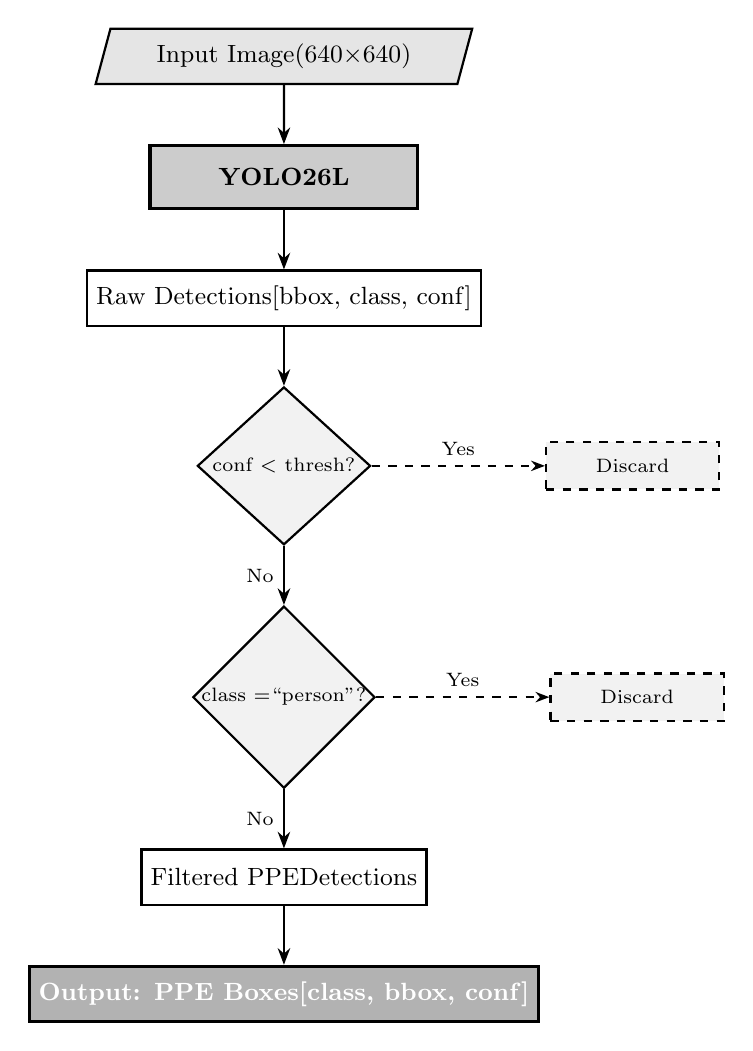
\begin{tikzpicture}[node distance=0.75cm and 2.2cm]

  % ── nodes ─────────────────────────────────────────────────────────────────
  \node[io]       (input)   {Input Image\\(640$\times$640)};
  \node[model,    below=of input]   (yolo)    {YOLO26L};
  \node[process,  below=of yolo]    (rawdet)  {Raw Detections\\{[bbox, class, conf]}};
  \node[decision, below=of rawdet]  (dconf)   {conf $<$ thresh?};
  \node[decision, below=of dconf]   (dperson) {class =\\``person''?};
  \node[process,  below=of dperson] (filtered){Filtered PPE\\Detections};
  \node[output,   below=of filtered](out)     {Output: PPE Boxes\\{[class, bbox, conf]}};

  % discard nodes (right side)
  \node[discard, right=of dconf]    (disc1)   {Discard};
  \node[discard, right=of dperson]  (disc2)   {Discard};

  % ── edges ─────────────────────────────────────────────────────────────────
  \draw[arr] (input)    -- (yolo);
  \draw[arr] (yolo)     -- (rawdet);
  \draw[arr] (rawdet)   -- (dconf);
  \draw[arr] (dconf)    -- node[left,  font=\scriptsize]{No}  (dperson);
  \draw[arr] (dperson)  -- node[left,  font=\scriptsize]{No}  (filtered);
  \draw[arr] (filtered) -- (out);

  \draw[darr](dconf)    -- node[above, font=\scriptsize]{Yes} (disc1);
  \draw[darr](dperson)  -- node[above, font=\scriptsize]{Yes} (disc2);

\end{tikzpicture}
\end{document}
